%%%%%%%%%%%%%%%%%%%%%%%%%%%%%%%%%%%%%%%%%
% Short Sectioned Assignment
% LaTeX Template
% Version 1.0 (5/5/12)
%
% This template has been downloaded from:
% http://www.LaTeXTemplates.com
%
% Original author:
% Frits Wenneker (http://www.howtotex.com)
%
% License:
% CC BY-NC-SA 3.0 (http://creativecommons.org/licenses/by-nc-sa/3.0/)
%
%%%%%%%%%%%%%%%%%%%%%%%%%%%%%%%%%%%%%%%%%

%----------------------------------------------------------------------------------------
%	PACKAGES AND OTHER DOCUMENT CONFIGURATIONS
%----------------------------------------------------------------------------------------

\documentclass[paper=a4, fontsize=12pt]{scrartcl} % A4 paper and 11pt font size

\usepackage[T1]{fontenc} % Use 8-bit encoding that has 256 glyphs
\usepackage{lmodern}

\usepackage[english]{babel} % English language/hyphenation
\usepackage{hyperref}

\setlength\parindent{0pt} % Removes all indentation from paragraphs - comment this line for an assignment with lots of text

%% own stuff
\usepackage{listings}
\usepackage{xcolor}
\definecolor{my-gray}{RGB}{224,224,224}
\lstset{
  breaklines=true,
  basicstyle=\small,
  columns=fullflexible,
  frame=lines,
  backgroundcolor=\color{my-gray} 
}

\colorlet{punct}{red!60!black}
\definecolor{background}{HTML}{EEEEEE}
\definecolor{delim}{RGB}{20,105,176}
\colorlet{numb}{magenta!60!black}

\lstdefinelanguage{json}{
    literate=
     *{0}{{{\color{numb}0}}}{1}
      {1}{{{\color{numb}1}}}{1}
      {2}{{{\color{numb}2}}}{1}
      {3}{{{\color{numb}3}}}{1}
      {4}{{{\color{numb}4}}}{1}
      {5}{{{\color{numb}5}}}{1}
      {6}{{{\color{numb}6}}}{1}
      {7}{{{\color{numb}7}}}{1}
      {8}{{{\color{numb}8}}}{1}
      {9}{{{\color{numb}9}}}{1}
      {:}{{{\color{punct}{:}}}}{1}
      {,}{{{\color{punct}{,}}}}{1}
      {\{}{{{\color{delim}{\{}}}}{1}
      {\}}{{{\color{delim}{\}}}}}{1}
      {[}{{{\color{delim}{[}}}}{1}
      {]}{{{\color{delim}{]}}}}{1},
}

\lstset{language=SQL,morekeywords={PREFIX,java,rdf,rdfs,url}}
\lstdefinelanguage{wsmo}{
  keywords={concept,annotations,endAnnotations,hasValue,ofType,relation,axiom,definedBy,forall,impliedBy,memberOf,instance}
}
\usepackage{graphicx}

%----------------------------------------------------------------------------------------
%	TITLE SECTION
%----------------------------------------------------------------------------------------

\newcommand{\horrule}[1]{\rule{\linewidth}{#1}} % Create horizontal rule command with 1 argument of height

\title{	
\normalfont \normalsize 
\textsc{University of Innsbruck} \\ [25pt] % Your university, school and/or department name(s)
\horrule{0.5pt} \\[0.4cm] % Thin top horizontal rule
\huge Semantic Web - Exercise sheet 4 \\ % The assignment title
\horrule{2pt} \\[0.5cm] % Thick bottom horizontal rule
}

\author{Jan Schlenker} % Your name

\date{\normalsize\today} % Today's date or a custom date

\begin{document}

\maketitle % Print the title

%----------------------------------------------------------------------------------------
%	PROBLEM 1
%----------------------------------------------------------------------------------------

\section{Exercise 1 (RDFa)}

The html document \texttt{events.html} contains the annotated initial html document. The corresponding, with \href{http://rdfa.info/play/}{http://rdfa.info/play/} generated graph is illustrated below:

\begin{figure}[htbp]
  \centering
  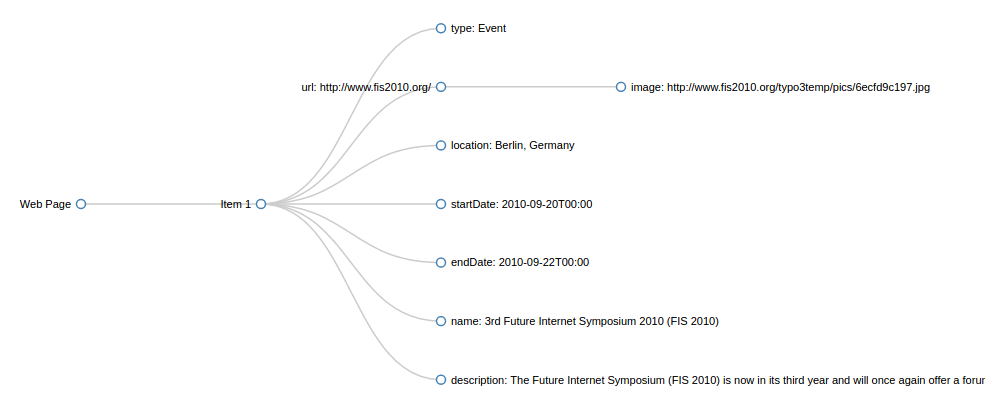
\includegraphics[width=\textwidth]{graph.png}
\end{figure}

The image node is probably wrongly generated. I tried different variations to get a proper visualization, but this is the best variation I found.


%----------------------------------------------------------------------------------------
%	PROBLEM 2
%----------------------------------------------------------------------------------------

\section{Exercise 3 (Linked Data Principles)}

Linked Data is one method (among others) to publish structured data. It is based on the standard web technologies \textbf{HTTP}, \textbf{URI} and \textbf{RDF}. Thus it can lower the entry barrier for data providers, which want to annotate their data and be part of the Semantic Web. \\
\\
The principles of Linked Data outlined by Tim Bernes-Lee (in 2006):

\textit{
\begin{itemize}
\item Use URIs to name (identify) things.
\item Use HTTP URIs so that these things can be looked up (interpreted, "dereferenced").
\item Provide useful information about what a name identifies when it's looked up, using open standards such as RDF, SPARQL, etc.
\item Refer to other things using their HTTP URI-based names when publishing data on the Web.
\end{itemize}
}

He restated this principles in 2009, so that they are even more simple:

\textit{
\begin{itemize}
\item All kinds of conceptual things, they have names now that start with HTTP.
\item If I take one of these HTTP names and I look it up...I will get back some data in a standard format which is kind of useful data that somebody might like to know about that thing, about that event.
\item When I get back that information it's not just got somebody's height and weight and when they were born, its got relationships. And when it has relationships, whenever it expresses a relationship then the other thing that it's related to is given one of those names that starts with HTTP.
\end{itemize}
}

\end{document}
